\begin{figure}[t]
\centering
\includegraphics[width=0.65\columnwidth]{images/varifocal_occlusion/prototype}
%\fbox{\includegraphics[width=0.46\textwidth]{images/prototype}}
\caption[varifocal-Occlusion NED: Benchtop prototype and staged real-world scene for capturing results]{\textit{(A)} Photo of our varifocal occlusion-capable AR display \textit{(B)} Optical design of the prototype. Static design parameters are denoted in green. Propagation of real-world light through the system is depicted with red arrows. Propagation of the virtual image is depicted with blue arrows. The arrows are only representative of the general direction of propagation and do not depict the exact path taken by the light rays. \textit{(C)} Photo of lab set-up which shows the prototype and the three real objects: stamp at 30cm, motorcycle at 100cm, and gnome at 300cm.}
\label{fig:varifocal_occlusion:prototype}
\end{figure}
